\documentclass[a4paper]{article}

%% Language and font encodings
\usepackage[english]{babel}
\usepackage[utf8x]{inputenc}
\usepackage[T1]{fontenc}

%% Useful packages
\usepackage{amsmath}
\usepackage{amssymb}
\usepackage{amsfonts} 
\usepackage{graphicx}
\usepackage{listings}
\usepackage{color}
\usepackage[colorinlistoftodos]{todonotes}
\usepackage[colorlinks=true, allcolors=blue]{hyperref}

%% Defining commands
\newcommand{\R}{\mathbb{R}}
\newcommand{\Z}{\mathbb{Z}}
\newcommand{\Q}{\mathbb{Q}}
\newcommand\tab[1][1cm]{\hspace*{#1}}
\newcommand*{\perm}[2]{{}^{#1}\!P_{#2}}%
\newcommand*{\comb}[2]{{}^{#1}C_{#2}}%

%% Sets page size and margins
\usepackage[a4paper,top=3cm,bottom=2cm,left=3cm,right=3cm,marginparwidth=1.75cm]{geometry}

%% Setting up code blocks
\lstset{frame=tb,
	aboveskip=3mm,
	belowskip=3mm,
	showstringspaces=false,
	columns=flexible,
	basicstyle={\small\ttfamily},
	numbers=none,
	breaklines=true,
	breakatwhitespace=true,
	tabsize=3
}




\title{%
	CS1231 Part 12 - Graphs, Continued  \\
	\large Based on lectures by Terence Sim and Aaron Tan
	\\ Notes taken by Andrew Tan
	\\ AY18/19 Semester 1
	\\ }

\author{}
\date{\vspace{-5ex}}

\begin{document}
\maketitle

\begin{center}\begin{minipage}[c]{0.9\textwidth}\centering\footnotesize These notes are not endorsed by the lecturers, and I have modified them (often significantly) after lectures. They are nowhere near accurate representations of what was actually lectured, and in particular, all errors are almost surely mine.\end{minipage}\end{center}

\section{Trees}
A graph is called a \textbf{tree} if, and only if, it has no circuits and is connected.\\\\
A \textbf{trivial tree} is a graph that consists of a single vertex.\\\\
A graph is called a \textbf{forest} if, and only if, it has no circuits and is not connected.

\subsubsection{Characterizing trees}
We begin with the following lemma:
\begin{itemize}
	\item[] Lemma 10.5.1 - Any non-trivial tree has at least one vertex of degree 1. 
\end{itemize}
We can easily show this is true simply by starting at any vertex and moving from one vertex to another without repetition until we reach a vertex of degree 1 (as there are no circuits).\\\\
In fact, we can use Lemma 10.5.1 to show that any tree with more than one vertex has at least \textit{two} vertices of degree 1.\\\\
We now obtain the following definitions: Let $T$ be a tree,
\begin{itemize}
	\item[] \textbf{Terminal vertex} or \textbf{leaf} - a vertex of degree 1 in $T$.
	\item[] \textbf{Internal vertex} - a vertex of degree greater than 1 in $T$.
\end{itemize}
And the following theorems and lemmas:
\begin{itemize}
	\item[] Theorem 10.5.2 - Any tree with $n$ vertices ($n>0$) has $n-1$ edges.
	\item[] Lemma 10.5.3 - If $G$ is any connected graph with $n$ vertices and $n-1$ edges, then $G$ is a tree.
	\item[] Theorem 10.5.4 - If $G$ is a connected graph with $n$ vertices and $n-1$ edges, then $G$ is a tree.
\end{itemize}
We can prove Theorem 10.5.2 with mathematical induction and with Lemma 10.5.1.\\\\
The intuition behind Lemma 10.5.3 is that any two vertices in a circuit are connected by two distinct paths, one going "clockwise", and the other going "counter-clockwise" around the circuit.\\\\
With this, we can prove Theorem 10.5.4 by first starting with an particular but arbitrarily chosen graph that is connected and has $n$ vertices and $n-1$ edges. We only need to show that $G$ does not contain a circuit (with the use of Lemma 10.5.3 and Theorem 10.5.2).

\section{Rooted Trees}
A \textbf{rooted tree} is a tree in which one vertex has been distinguished from the others and is designated the \textbf{root}. Furthermore, the \textbf{level} of a vertex is the number of edges along the unique path between it and the root, and the \textbf{height} of a rooted tree is the maximum level of any vertex of the tree.\\\\
Given the root or any internal vertex $v$ of a rooted tree, the \textbf{children} of $v$ are all those vertices that are adjacent to $v$ and are one level farther away from the root than $v$.\\\\
If $w$ is a child of $v$, then $v$ is called the parent of $w$, and two distinct vertices that are both children of the same parent are called \textbf{siblings}. \\\\
Furthermore, given two distinct vertices of $v$ and $w$, if $v$ lies on the unique path between $w$ and the root, then $v$ is an \textbf{ancestor} of $w$, and $w$ is a \textbf{descendant} of $v$.

\subsubsection{Binary trees}
A \textbf{binary tree} is a rooted tree in which every parent has at most two children. Each child is designated either a \textbf{left child} or a \textbf{right child} (but not both), and every parent has at most one left child and one right child.\\\\
A \textbf{full binary tree} is a binary tree in which each parent has exactly two children.\\\\
Furthermore, given any parent $v$ in a binary tree $T$, if $v$ has a left child, then the \textbf{left subtree} of $v$ is the binary tree whose root is the left child of $v$, whose vertices consist of the left child of $v$ and all its descendants, and whose edges consist of all those edges of $T$ that conect the vertices of the left subtree. The \textbf{right subtree} of $v$ is defined analogously.\\\\
If we know the number of internal vertices of a full binary tree, then we can calculate both the total number of vertices and the number of terminal vertices (leaves), and conversely:
\begin{itemize}
	\item[] Theorem 10.6.1 - If $T$ is a full binary tree with $k$ internal vertices, then $T$ has a total of $2k+1$ vertices and has $k+1$ terminal vertices. 
\end{itemize}
Furthermore, for any binary tree, we can calculate the upper bound of the number of leaves of the binary tree:
\begin{itemize}
	\item[] Theorem 10.6.2 - For non-negative integers $h$, if $T$ is any binary tree with height $h$ and $t$ leaves, then
	\begin{center}
		$t\le 2^h$, or equivalently, $\log_2{t} \le h$
	\end{center}
\end{itemize}

\subsection{Binary tree traversal}
\textbf{Tree traversal} of \textbf{tree search} is the process of visiting each node in a tree data structure exactly once in a systematic manner.\\\\
We will be studying two types of traversal: \textbf{breadth-first search (BFS)} or \textbf{depth-first search (DFS)}.\\\\
The following section describe BFS and DFS on binary trees, but in general they can be applied on any graphs.

\subsubsection{Breadth-first search}
In breadth-first search, it starts at the root and visits its adjacent vertices, and then moves to the next level. Essentially, we explore all the nodes at the current level, before we move to the next level and repeat the process.\\\\\\
This figure shows a possible order of the vertices visited in the given binary tree.
\begin{center}
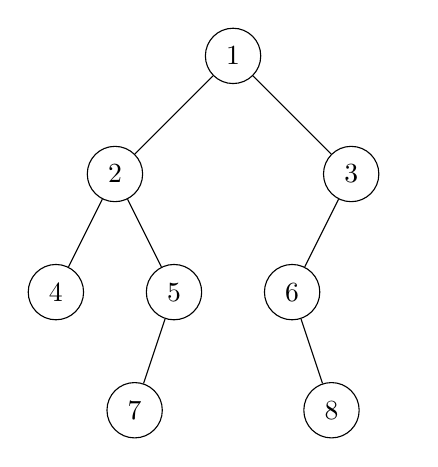
\begin{tikzpicture}[
	every node/.style = {minimum width = 2em, draw, circle},
	level/.style = {sibling distance = 30mm/#1}
	]
	\node {1}
	child {node {2} 
		child {node {4}}
		child {node {5}
			child {node {7}}
			child {edge from parent[draw = none]}
		}
	}
	child {node {3}
		child {node {6}
			child {edge from parent[draw = none]}
			child {node {8}}
		}
		child {edge from parent[draw = none]}
	};
\end{tikzpicture}
\end{center}

\subsubsection{Depth-first search}
In depth-first search, we start at the root node and explore as deep as possible before backtracking.\\\\
There are three types of depth-first traversal:
\begin{itemize}
	\item \textbf{Pre-order}
	\begin{itemize}
		\item Print the data of the current vertex
		\item Traverse the left subtree by recursively calling the pre-order function
		\item Traverse the right subtree by recursively calling the pre-order function
	\end{itemize}
	\item \textbf{In-order}
	\begin{itemize}
		\item Traverse the left subtree by recursively calling the in-order function
		\item Print the data of the current vertex
		\item Traverse the right subtree by recursively calling the in-order function
	\end{itemize}
	\item \textbf{Post-order}
	\begin{itemize}
		\item Traverse the left subtree by recursively calling the post-order function
		\item Traverse the right subtree by recursively calling the post-order function
		\item Print the data of the current vertex
	\end{itemize}
\end{itemize}
Let's take a look at this tree:
\begin{center}
	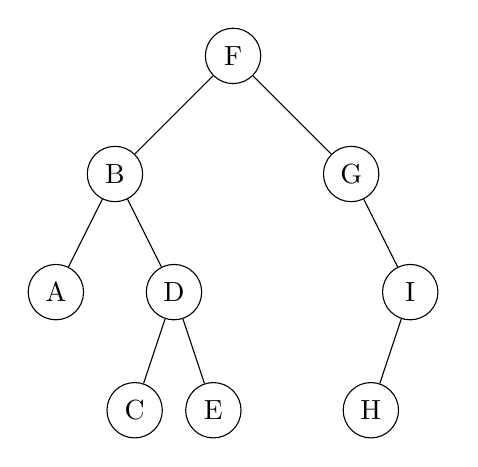
\begin{tikzpicture}[
	every node/.style = {minimum width = 2em, draw, circle},
	level/.style = {sibling distance = 30mm/#1}
	]
	\node {F}
	child {node {B} 
		child {node {A}}
		child {node {D}
			child {node {C}}
			child {node {E}}
		}
	}
	child {node {G}
		child {edge from parent[draw = none]}
		child {node {I}
			child {node {H}}
			child{edge from parent[draw = none]}		
		}
	};
	\end{tikzpicture}
\end{center}
Pre-order: F, B, A, D, C, E, G, I, H\\
In-order: A, B, C, D, E, F, G, H, I\\
Post-order: A, C, E, D, B, H, I, G, F

\section{Spanning trees and shortest paths}
A \textbf{spanning tree} for a graph $G$ is a subgraph of $G$ that contains every vertex of $G$ and is a tree.
\begin{itemize}
	\item[] Proposition 10.7.1 - 
	\begin{enumerate}
		\item Every connected graph has a spanning tree.
		\item Any two spanning trees for a graph have the same number of edges.
	\end{enumerate}
\end{itemize}

\subsection{Minimum spanning trees}
A \textbf{weighted graph} is a graph for which each edge has an associated positive real number \textbf{weight} . The sum of the weights of all the edges is the \textbf{total weight} of the graph.\\\\
A \textbf{minimum spanning tree} for a connected weighted graph is a spanning tree that has the least possible total weight compared to all other spanning trees for the graph.\\\\
If $G$ is a weighted graph and $e$ is an edge of $G$, then $w(e)$ denotes the weight of $e$ and $w(G)$ denotes the total weight of $G$.\\\\
We explore two algorithms that help us to construct a minimum spanning tree:

\subsubsection{Kruskal's algorithm}
In \textbf{Kruskal’s algorithm}, the edges of a connected weighted graph are examined one by one in order of increasing weight.\\\\ 
At each stage the edge being examined is added to what will become the minimum spanning tree, provided that this addition does not create a circuit.\\\\
After $n$–$1$ edges have been added (where $n$ is the number of vertices of the graph), these edges, together with the vertices of the graph, form a minimum spanning tree for the graph.\\\\
We sketch Kruskal's algorithm as follows:\\
Input: $G$ (a connected weighted graph with $n$ vertices)
\begin{enumerate}
	\item Initialize $T$ to have all the vertices of $G$ and no edges.
	\item Let $E$ be the set of all edges of $G$, and let $m=0$.
	\item While $(m<n-1)$
	\begin{enumerate}
		\item Find an edge $e$ in $E$ of least weight.
		\item Delete $e$ from $E$.
		\item If addition of $e$ to the edge set of $T$ does not produce a circuit, then add $e$ to the edge set of $T$ and set $m=m+1$.
	\end{enumerate}
\end{enumerate}
Output: $T$ (a minimum spanning tree for $G$)

\subsubsection{Prim's algorithm}
In \textbf{Prim's algorithm}, it builds a minimum spanning tree by expanding outward in connected links from some vertex.\\\\
One edge and one vertex are added at each stage. The edge added is the one of least weight that connects the vertices already in $T$ with those not in $T$, and the vertex is the endpoint of this edge that is not already in $T$.\\\\
We sketch Prim's algorithm as follows:\\
Input: $G$ (a connected weighted graph with $n$ vertices)
\begin{enumerate}
	\item Pick a vertex $v$ of $G$ and let $T$ be the graph with this vertex only.
	\item Let $V$ be the set of all vertices of $G$ except $v$
	\item For $i=1$ to $n-1$
	\begin{enumerate}
		\item Find an edge $e$ of $G$ such that (1) $e$ connects $T$ to one of the vertices in $V$, and (2) $e$ has the least weight of all edges connecting $T$ to a vertex in $V$. Let $w$ be the endpoint of $e$ that is in $V$.
		\item Add $e$ and $w$ to the edge and vertex sets of $T$, and delete $w$ from $V$.
	\end{enumerate}
\end{enumerate}
Output: $T$ (a minimum spanning tree for $G$)

\subsection{Dijkstra's shortest path}
In 1959, Edsgar Dijkstra developed an algorithm to find the shortest path between a starting vertex (source) and an ending vertex (destination) in a weighted graph in which all weights are positive.\\\\
Somewhat similar to Prim’s algorithms, it works outward from the source $a$, adding vertices and edges one by one to construct a shortest path tree $T$. It differs from Prim’s algorithm in the way it chooses the next vertex to add, ensuring that for each added vertex $v$, the length of the shortest path from $a$ to $v$ has been identified.\\\\
Intuition behind Dijkstra's algorithm:
\begin{itemize}
	\item Report the vertices in increasing order of their distance from the source vertex.
	\item Construct the shortest path tree edge by edge; at each step addingn one new edge, corresponding to construction of the sortest path to the current new vertex.
\end{itemize}
We sketch Dijkstra's algorithm as follows:\\
Inputs: 
\begin{itemize}
	\itemsep -0.5em
	\item $G$ (a connected simple graph with positive weight for every edge)
	\item $\infty$ (a number greater than the sum of the weights of all the edges in $G$)
	\item $w(u,v)$ (the weight of edge {$u,v$})
	\item $a$ (the source vertex)
	\item $z$ (the destination vertex)
\end{itemize}
\begin{enumerate}
	\item Initialize $T$ to be the graph with vertex $a$ and no edges. Let $V(T)$ be the set of vertices of $T$, and let $E(T)$ be the set of edges of $T$.
	\item $L(a) \leftarrow 0$, and for all vertices $u$ in $G$ except $a$, $L(u) \leftarrow \infty$ (The number $L(u)$ is called the \textit{label} of $u$.
	\item Initialize $v \leftarrow a$ and $F\leftarrow \{a\}$. (the symbol $v$ is used to denote the vertex most recently added to $T$).
	\item[] Let $Adj(x)$ denote the set of vertices adjacent to vertex $x$
	\item while $(z\notin V(T))$
	\begin{enumerate}
		\item $F\leftarrow (F-\{v\}) \cup \{vertices \in Adj(v)$ and $\notin V(T)\}$ (The set $F$ is the set of \textit{fringe vertices, i.e. the vertices adjacent to at least one vertex of $T$ but are not in $T$})
		\item For each vertex $u \in Adj(v)$ and $\notin V(T)$\\
		if $L(v) + w(v, u) < L(u)$ then
		\begin{itemize}
			\item[] $L(u) \leftarrow L(v) + w(v,u)$
			\item[] $D(u) \leftarrow v$, where $D(u)$ is used to keep track of which vertex in $T$ gave rise to the smaller value.
		\end{itemize}
		\item Find a vertex $x$ in $F$ with the smallest label. Add vertex $x$ to $V(T)$, and add edge $\{D(x), x\}$ to $E(T)$.\\
		$v\leftarrow x$
	\end{enumerate}
\end{enumerate}
Output: $L(z)$ (the length of the shortest path from $a$ to $z$).


\end{document}